\documentclass[10pt]{article}
\usepackage[preprint]{tmlr}
%%%%% NEW MATH DEFINITIONS %%%%%

\usepackage{amsmath,amsfonts,bm}

% Mark sections of captions for referring to divisions of figures
\newcommand{\figleft}{{\em (Left)}}
\newcommand{\figcenter}{{\em (Center)}}
\newcommand{\figright}{{\em (Right)}}
\newcommand{\figtop}{{\em (Top)}}
\newcommand{\figbottom}{{\em (Bottom)}}
\newcommand{\captiona}{{\em (a)}}
\newcommand{\captionb}{{\em (b)}}
\newcommand{\captionc}{{\em (c)}}
\newcommand{\captiond}{{\em (d)}}

% Highlight a newly defined term
\newcommand{\newterm}[1]{{\bf #1}}


% Figure reference, lower-case.
\def\figref#1{figure~\ref{#1}}
% Figure reference, capital. For start of sentence
\def\Figref#1{Figure~\ref{#1}}
\def\twofigref#1#2{figures \ref{#1} and \ref{#2}}
\def\quadfigref#1#2#3#4{figures \ref{#1}, \ref{#2}, \ref{#3} and \ref{#4}}
% Section reference, lower-case.
\def\secref#1{section~\ref{#1}}
% Section reference, capital.
\def\Secref#1{Section~\ref{#1}}
% Reference to two sections.
\def\twosecrefs#1#2{sections \ref{#1} and \ref{#2}}
% Reference to three sections.
\def\secrefs#1#2#3{sections \ref{#1}, \ref{#2} and \ref{#3}}
% Reference to an equation, lower-case.
\def\eqref#1{equation~\ref{#1}}
% Reference to an equation, upper case
\def\Eqref#1{Equation~\ref{#1}}
% A raw reference to an equation---avoid using if possible
\def\plaineqref#1{\ref{#1}}
% Reference to a chapter, lower-case.
\def\chapref#1{chapter~\ref{#1}}
% Reference to an equation, upper case.
\def\Chapref#1{Chapter~\ref{#1}}
% Reference to a range of chapters
\def\rangechapref#1#2{chapters\ref{#1}--\ref{#2}}
% Reference to an algorithm, lower-case.
\def\algref#1{algorithm~\ref{#1}}
% Reference to an algorithm, upper case.
\def\Algref#1{Algorithm~\ref{#1}}
\def\twoalgref#1#2{algorithms \ref{#1} and \ref{#2}}
\def\Twoalgref#1#2{Algorithms \ref{#1} and \ref{#2}}
% Reference to a part, lower case
\def\partref#1{part~\ref{#1}}
% Reference to a part, upper case
\def\Partref#1{Part~\ref{#1}}
\def\twopartref#1#2{parts \ref{#1} and \ref{#2}}

\def\ceil#1{\lceil #1 \rceil}
\def\floor#1{\lfloor #1 \rfloor}
\def\1{\bm{1}}
\newcommand{\train}{\mathcal{D}}
\newcommand{\valid}{\mathcal{D_{\mathrm{valid}}}}
\newcommand{\test}{\mathcal{D_{\mathrm{test}}}}

\def\eps{{\epsilon}}


% Random variables
\def\reta{{\textnormal{$\eta$}}}
\def\ra{{\textnormal{a}}}
\def\rb{{\textnormal{b}}}
\def\rc{{\textnormal{c}}}
\def\rd{{\textnormal{d}}}
\def\re{{\textnormal{e}}}
\def\rf{{\textnormal{f}}}
\def\rg{{\textnormal{g}}}
\def\rh{{\textnormal{h}}}
\def\ri{{\textnormal{i}}}
\def\rj{{\textnormal{j}}}
\def\rk{{\textnormal{k}}}
\def\rl{{\textnormal{l}}}
% rm is already a command, just don't name any random variables m
\def\rn{{\textnormal{n}}}
\def\ro{{\textnormal{o}}}
\def\rp{{\textnormal{p}}}
\def\rq{{\textnormal{q}}}
\def\rr{{\textnormal{r}}}
\def\rs{{\textnormal{s}}}
\def\rt{{\textnormal{t}}}
\def\ru{{\textnormal{u}}}
\def\rv{{\textnormal{v}}}
\def\rw{{\textnormal{w}}}
\def\rx{{\textnormal{x}}}
\def\ry{{\textnormal{y}}}
\def\rz{{\textnormal{z}}}

% Random vectors
\def\rvepsilon{{\mathbf{\epsilon}}}
\def\rvtheta{{\mathbf{\theta}}}
\def\rva{{\mathbf{a}}}
\def\rvb{{\mathbf{b}}}
\def\rvc{{\mathbf{c}}}
\def\rvd{{\mathbf{d}}}
\def\rve{{\mathbf{e}}}
\def\rvf{{\mathbf{f}}}
\def\rvg{{\mathbf{g}}}
\def\rvh{{\mathbf{h}}}
\def\rvu{{\mathbf{i}}}
\def\rvj{{\mathbf{j}}}
\def\rvk{{\mathbf{k}}}
\def\rvl{{\mathbf{l}}}
\def\rvm{{\mathbf{m}}}
\def\rvn{{\mathbf{n}}}
\def\rvo{{\mathbf{o}}}
\def\rvp{{\mathbf{p}}}
\def\rvq{{\mathbf{q}}}
\def\rvr{{\mathbf{r}}}
\def\rvs{{\mathbf{s}}}
\def\rvt{{\mathbf{t}}}
\def\rvu{{\mathbf{u}}}
\def\rvv{{\mathbf{v}}}
\def\rvw{{\mathbf{w}}}
\def\rvx{{\mathbf{x}}}
\def\rvy{{\mathbf{y}}}
\def\rvz{{\mathbf{z}}}

% Elements of random vectors
\def\erva{{\textnormal{a}}}
\def\ervb{{\textnormal{b}}}
\def\ervc{{\textnormal{c}}}
\def\ervd{{\textnormal{d}}}
\def\erve{{\textnormal{e}}}
\def\ervf{{\textnormal{f}}}
\def\ervg{{\textnormal{g}}}
\def\ervh{{\textnormal{h}}}
\def\ervi{{\textnormal{i}}}
\def\ervj{{\textnormal{j}}}
\def\ervk{{\textnormal{k}}}
\def\ervl{{\textnormal{l}}}
\def\ervm{{\textnormal{m}}}
\def\ervn{{\textnormal{n}}}
\def\ervo{{\textnormal{o}}}
\def\ervp{{\textnormal{p}}}
\def\ervq{{\textnormal{q}}}
\def\ervr{{\textnormal{r}}}
\def\ervs{{\textnormal{s}}}
\def\ervt{{\textnormal{t}}}
\def\ervu{{\textnormal{u}}}
\def\ervv{{\textnormal{v}}}
\def\ervw{{\textnormal{w}}}
\def\ervx{{\textnormal{x}}}
\def\ervy{{\textnormal{y}}}
\def\ervz{{\textnormal{z}}}

% Random matrices
\def\rmA{{\mathbf{A}}}
\def\rmB{{\mathbf{B}}}
\def\rmC{{\mathbf{C}}}
\def\rmD{{\mathbf{D}}}
\def\rmE{{\mathbf{E}}}
\def\rmF{{\mathbf{F}}}
\def\rmG{{\mathbf{G}}}
\def\rmH{{\mathbf{H}}}
\def\rmI{{\mathbf{I}}}
\def\rmJ{{\mathbf{J}}}
\def\rmK{{\mathbf{K}}}
\def\rmL{{\mathbf{L}}}
\def\rmM{{\mathbf{M}}}
\def\rmN{{\mathbf{N}}}
\def\rmO{{\mathbf{O}}}
\def\rmP{{\mathbf{P}}}
\def\rmQ{{\mathbf{Q}}}
\def\rmR{{\mathbf{R}}}
\def\rmS{{\mathbf{S}}}
\def\rmT{{\mathbf{T}}}
\def\rmU{{\mathbf{U}}}
\def\rmV{{\mathbf{V}}}
\def\rmW{{\mathbf{W}}}
\def\rmX{{\mathbf{X}}}
\def\rmY{{\mathbf{Y}}}
\def\rmZ{{\mathbf{Z}}}

% Elements of random matrices
\def\ermA{{\textnormal{A}}}
\def\ermB{{\textnormal{B}}}
\def\ermC{{\textnormal{C}}}
\def\ermD{{\textnormal{D}}}
\def\ermE{{\textnormal{E}}}
\def\ermF{{\textnormal{F}}}
\def\ermG{{\textnormal{G}}}
\def\ermH{{\textnormal{H}}}
\def\ermI{{\textnormal{I}}}
\def\ermJ{{\textnormal{J}}}
\def\ermK{{\textnormal{K}}}
\def\ermL{{\textnormal{L}}}
\def\ermM{{\textnormal{M}}}
\def\ermN{{\textnormal{N}}}
\def\ermO{{\textnormal{O}}}
\def\ermP{{\textnormal{P}}}
\def\ermQ{{\textnormal{Q}}}
\def\ermR{{\textnormal{R}}}
\def\ermS{{\textnormal{S}}}
\def\ermT{{\textnormal{T}}}
\def\ermU{{\textnormal{U}}}
\def\ermV{{\textnormal{V}}}
\def\ermW{{\textnormal{W}}}
\def\ermX{{\textnormal{X}}}
\def\ermY{{\textnormal{Y}}}
\def\ermZ{{\textnormal{Z}}}

% Vectors
\def\vzero{{\bm{0}}}
\def\vone{{\bm{1}}}
\def\vmu{{\bm{\mu}}}
\def\vtheta{{\bm{\theta}}}
\def\va{{\bm{a}}}
\def\vb{{\bm{b}}}
\def\vc{{\bm{c}}}
\def\vd{{\bm{d}}}
\def\ve{{\bm{e}}}
\def\vf{{\bm{f}}}
\def\vg{{\bm{g}}}
\def\vh{{\bm{h}}}
\def\vi{{\bm{i}}}
\def\vj{{\bm{j}}}
\def\vk{{\bm{k}}}
\def\vl{{\bm{l}}}
\def\vm{{\bm{m}}}
\def\vn{{\bm{n}}}
\def\vo{{\bm{o}}}
\def\vp{{\bm{p}}}
\def\vq{{\bm{q}}}
\def\vr{{\bm{r}}}
\def\vs{{\bm{s}}}
\def\vt{{\bm{t}}}
\def\vu{{\bm{u}}}
\def\vv{{\bm{v}}}
\def\vw{{\bm{w}}}
\def\vx{{\bm{x}}}
\def\vy{{\bm{y}}}
\def\vz{{\bm{z}}}

% Elements of vectors
\def\evalpha{{\alpha}}
\def\evbeta{{\beta}}
\def\evepsilon{{\epsilon}}
\def\evlambda{{\lambda}}
\def\evomega{{\omega}}
\def\evmu{{\mu}}
\def\evpsi{{\psi}}
\def\evsigma{{\sigma}}
\def\evtheta{{\theta}}
\def\eva{{a}}
\def\evb{{b}}
\def\evc{{c}}
\def\evd{{d}}
\def\eve{{e}}
\def\evf{{f}}
\def\evg{{g}}
\def\evh{{h}}
\def\evi{{i}}
\def\evj{{j}}
\def\evk{{k}}
\def\evl{{l}}
\def\evm{{m}}
\def\evn{{n}}
\def\evo{{o}}
\def\evp{{p}}
\def\evq{{q}}
\def\evr{{r}}
\def\evs{{s}}
\def\evt{{t}}
\def\evu{{u}}
\def\evv{{v}}
\def\evw{{w}}
\def\evx{{x}}
\def\evy{{y}}
\def\evz{{z}}

% Matrix
\def\mA{{\bm{A}}}
\def\mB{{\bm{B}}}
\def\mC{{\bm{C}}}
\def\mD{{\bm{D}}}
\def\mE{{\bm{E}}}
\def\mF{{\bm{F}}}
\def\mG{{\bm{G}}}
\def\mH{{\bm{H}}}
\def\mI{{\bm{I}}}
\def\mJ{{\bm{J}}}
\def\mK{{\bm{K}}}
\def\mL{{\bm{L}}}
\def\mM{{\bm{M}}}
\def\mN{{\bm{N}}}
\def\mO{{\bm{O}}}
\def\mP{{\bm{P}}}
\def\mQ{{\bm{Q}}}
\def\mR{{\bm{R}}}
\def\mS{{\bm{S}}}
\def\mT{{\bm{T}}}
\def\mU{{\bm{U}}}
\def\mV{{\bm{V}}}
\def\mW{{\bm{W}}}
\def\mX{{\bm{X}}}
\def\mY{{\bm{Y}}}
\def\mZ{{\bm{Z}}}
\def\mBeta{{\bm{\beta}}}
\def\mPhi{{\bm{\Phi}}}
\def\mLambda{{\bm{\Lambda}}}
\def\mSigma{{\bm{\Sigma}}}

% Tensor
\DeclareMathAlphabet{\mathsfit}{\encodingdefault}{\sfdefault}{m}{sl}
\SetMathAlphabet{\mathsfit}{bold}{\encodingdefault}{\sfdefault}{bx}{n}
\newcommand{\tens}[1]{\bm{\mathsfit{#1}}}
\def\tA{{\tens{A}}}
\def\tB{{\tens{B}}}
\def\tC{{\tens{C}}}
\def\tD{{\tens{D}}}
\def\tE{{\tens{E}}}
\def\tF{{\tens{F}}}
\def\tG{{\tens{G}}}
\def\tH{{\tens{H}}}
\def\tI{{\tens{I}}}
\def\tJ{{\tens{J}}}
\def\tK{{\tens{K}}}
\def\tL{{\tens{L}}}
\def\tM{{\tens{M}}}
\def\tN{{\tens{N}}}
\def\tO{{\tens{O}}}
\def\tP{{\tens{P}}}
\def\tQ{{\tens{Q}}}
\def\tR{{\tens{R}}}
\def\tS{{\tens{S}}}
\def\tT{{\tens{T}}}
\def\tU{{\tens{U}}}
\def\tV{{\tens{V}}}
\def\tW{{\tens{W}}}
\def\tX{{\tens{X}}}
\def\tY{{\tens{Y}}}
\def\tZ{{\tens{Z}}}


% Graph
\def\gA{{\mathcal{A}}}
\def\gB{{\mathcal{B}}}
\def\gC{{\mathcal{C}}}
\def\gD{{\mathcal{D}}}
\def\gE{{\mathcal{E}}}
\def\gF{{\mathcal{F}}}
\def\gG{{\mathcal{G}}}
\def\gH{{\mathcal{H}}}
\def\gI{{\mathcal{I}}}
\def\gJ{{\mathcal{J}}}
\def\gK{{\mathcal{K}}}
\def\gL{{\mathcal{L}}}
\def\gM{{\mathcal{M}}}
\def\gN{{\mathcal{N}}}
\def\gO{{\mathcal{O}}}
\def\gP{{\mathcal{P}}}
\def\gQ{{\mathcal{Q}}}
\def\gR{{\mathcal{R}}}
\def\gS{{\mathcal{S}}}
\def\gT{{\mathcal{T}}}
\def\gU{{\mathcal{U}}}
\def\gV{{\mathcal{V}}}
\def\gW{{\mathcal{W}}}
\def\gX{{\mathcal{X}}}
\def\gY{{\mathcal{Y}}}
\def\gZ{{\mathcal{Z}}}

% Sets
\def\sA{{\mathbb{A}}}
\def\sB{{\mathbb{B}}}
\def\sC{{\mathbb{C}}}
\def\sD{{\mathbb{D}}}
% Don't use a set called E, because this would be the same as our symbol
% for expectation.
\def\sF{{\mathbb{F}}}
\def\sG{{\mathbb{G}}}
\def\sH{{\mathbb{H}}}
\def\sI{{\mathbb{I}}}
\def\sJ{{\mathbb{J}}}
\def\sK{{\mathbb{K}}}
\def\sL{{\mathbb{L}}}
\def\sM{{\mathbb{M}}}
\def\sN{{\mathbb{N}}}
\def\sO{{\mathbb{O}}}
\def\sP{{\mathbb{P}}}
\def\sQ{{\mathbb{Q}}}
\def\sR{{\mathbb{R}}}
\def\sS{{\mathbb{S}}}
\def\sT{{\mathbb{T}}}
\def\sU{{\mathbb{U}}}
\def\sV{{\mathbb{V}}}
\def\sW{{\mathbb{W}}}
\def\sX{{\mathbb{X}}}
\def\sY{{\mathbb{Y}}}
\def\sZ{{\mathbb{Z}}}

% Entries of a matrix
\def\emLambda{{\Lambda}}
\def\emA{{A}}
\def\emB{{B}}
\def\emC{{C}}
\def\emD{{D}}
\def\emE{{E}}
\def\emF{{F}}
\def\emG{{G}}
\def\emH{{H}}
\def\emI{{I}}
\def\emJ{{J}}
\def\emK{{K}}
\def\emL{{L}}
\def\emM{{M}}
\def\emN{{N}}
\def\emO{{O}}
\def\emP{{P}}
\def\emQ{{Q}}
\def\emR{{R}}
\def\emS{{S}}
\def\emT{{T}}
\def\emU{{U}}
\def\emV{{V}}
\def\emW{{W}}
\def\emX{{X}}
\def\emY{{Y}}
\def\emZ{{Z}}
\def\emSigma{{\Sigma}}

% entries of a tensor
% Same font as tensor, without \bm wrapper
\newcommand{\etens}[1]{\mathsfit{#1}}
\def\etLambda{{\etens{\Lambda}}}
\def\etA{{\etens{A}}}
\def\etB{{\etens{B}}}
\def\etC{{\etens{C}}}
\def\etD{{\etens{D}}}
\def\etE{{\etens{E}}}
\def\etF{{\etens{F}}}
\def\etG{{\etens{G}}}
\def\etH{{\etens{H}}}
\def\etI{{\etens{I}}}
\def\etJ{{\etens{J}}}
\def\etK{{\etens{K}}}
\def\etL{{\etens{L}}}
\def\etM{{\etens{M}}}
\def\etN{{\etens{N}}}
\def\etO{{\etens{O}}}
\def\etP{{\etens{P}}}
\def\etQ{{\etens{Q}}}
\def\etR{{\etens{R}}}
\def\etS{{\etens{S}}}
\def\etT{{\etens{T}}}
\def\etU{{\etens{U}}}
\def\etV{{\etens{V}}}
\def\etW{{\etens{W}}}
\def\etX{{\etens{X}}}
\def\etY{{\etens{Y}}}
\def\etZ{{\etens{Z}}}

% The true underlying data generating distribution
\newcommand{\pdata}{p_{\rm{data}}}
% The empirical distribution defined by the training set
\newcommand{\ptrain}{\hat{p}_{\rm{data}}}
\newcommand{\Ptrain}{\hat{P}_{\rm{data}}}
% The model distribution
\newcommand{\pmodel}{p_{\rm{model}}}
\newcommand{\Pmodel}{P_{\rm{model}}}
\newcommand{\ptildemodel}{\tilde{p}_{\rm{model}}}
% Stochastic autoencoder distributions
\newcommand{\pencode}{p_{\rm{encoder}}}
\newcommand{\pdecode}{p_{\rm{decoder}}}
\newcommand{\precons}{p_{\rm{reconstruct}}}

\newcommand{\laplace}{\mathrm{Laplace}} % Laplace distribution

\newcommand{\E}{\mathbb{E}}
\newcommand{\Ls}{\mathcal{L}}
\newcommand{\R}{\mathbb{R}}
\newcommand{\emp}{\tilde{p}}
\newcommand{\lr}{\alpha}
\newcommand{\reg}{\lambda}
\newcommand{\rect}{\mathrm{rectifier}}
\newcommand{\softmax}{\mathrm{softmax}}
\newcommand{\sigmoid}{\sigma}
\newcommand{\softplus}{\zeta}
\newcommand{\KL}{D_{\mathrm{KL}}}
\newcommand{\Var}{\mathrm{Var}}
\newcommand{\standarderror}{\mathrm{SE}}
\newcommand{\Cov}{\mathrm{Cov}}
% Wolfram Mathworld says $L^2$ is for function spaces and $\ell^2$ is for vectors
% But then they seem to use $L^2$ for vectors throughout the site, and so does
% wikipedia.
\newcommand{\normlzero}{L^0}
\newcommand{\normlone}{L^1}
\newcommand{\normltwo}{L^2}
\newcommand{\normlp}{L^p}
\newcommand{\normmax}{L^\infty}

\newcommand{\parents}{Pa} % See usage in notation.tex. Chosen to match Daphne's book.

\DeclareMathOperator*{\argmax}{arg\,max}
\DeclareMathOperator*{\argmin}{arg\,min}

\DeclareMathOperator{\sign}{sign}
\DeclareMathOperator{\Tr}{Tr}
\let\ab\allowbreak

\usepackage{amsmath,amssymb,bm,booktabs,tabularx,graphicx}
\usepackage{microtype,enumitem,placeins,float}
\usepackage{hyperref,url}
\hypersetup{
  hidelinks,
  pdftitle={Matched Specialization, Different Adaptation: Second-Moment Structure in Shared Representations},
  pdfauthor={Toru Takahashi}
}
\title{Matched Specialization, Different Adaptation:\\Second-Moment Structure in Shared Representations}
\author{\name Toru Takahashi \\
        \addr Human Informatics and Systems Lab, Doshisha University \\
        Linked Open Data Initiative, NPO \\
        Keio Research Institute at SFC \\
        Stroly Inc.}
\def\month{10}
\def\year{2026}
\newcommand{\figlang}{en}
\newif\ifpublicrelease
\publicreleasetrue
\begin{document}
\raggedbottom
\maketitle
\begingroup
\renewcommand{\thefootnote}{*}
\footnotetext{Generative AI assisted experiment design, implementation, analysis, literature work, and writing; see the AI assistance statement.}
\endgroup
\graphicspath{{../figures/}}
\begin{abstract}
% P:abstractnew
Small Adam-trained shared-representation networks can reach equivalent selected mean readout measurements yet respond differently to the same further learning. We use state interventions to separate second-moment scale and coordinate-pattern effects, then examine their formation and time dependence. In the central two-target experiment, the more precisely readable target switches within ten updates in 67.5\% of acquisition-formed checkpoints and 0\% of update-formed checkpoints. First-moment exchange leaves the ten-update contrast change within its pre-specified margin, whereas second-moment exchange reverses the contrast. A coordinate-pattern effect remains at common mean adaptive scale. Layer and movement controls locate an effect beyond overall update size. Formation records connect small encoder second moments with stronger cancellation between task gradients. A prospective gradient-projection experiment changes this retained state; transferring the resulting second moment alone reduces the ten-update adaptation response in a fixed recipient. The matched comparison extends to three Gaussian targets, while a room-sensor extension retains component effects but fails endpoint matching. Across tested regimes, component effects survive more widely than reversal or reset equivalence. Effect magnitude and duration depend on learning conditions.

\end{abstract}

\section{Introduction}
\label{sec:intro}
% P:introquestion
A shared representation supports several prediction tasks, yet limited capacity can make some targets easier to recover than others. We call this inequality in readout precision \emph{representational specialization}. Feature complexity, learning order, and competition between information sources can all produce such biases \citep{lampinen2024biased,pezeshki2021gradient,huang2022modality}. What remains uncertain is whether measuring this specialization also characterizes how readily it will change.

% P:introstakes
This question matters when a model resumes learning after evaluation. Similar current readout quality could coexist with different reallocation of shared features under the same future condition. Training history can affect later plasticity through both weights and optimizer state \citep{achille2019critical,lyle2023plasticity,dohare2024plasticity}. A useful comparison must first separate current measured ability from subsequent response, then intervene on a retained component without changing the recipient weights at the start.

% P:introcontribution
We build this comparison through two routes: observing one target more precisely, or assigning its reconstruction error more weight. After pilot calibration and independent confirmation of selected endpoint measurements, a common opposing condition reveals a large early response difference. We call the difference concealed by those measurements \emph{latent susceptibility}. The contribution is to separate second-moment scale from coordinate pattern at matched readouts and connect these response effects to their formation. Finally, changed networks, three targets, and longer continuations distinguish the component effect from the narrower conditions for reversal or reset equivalence.

\section{Relation to training history and optimizer memory}
\label{sec:related}
% P:related1
Similar measured performance can coexist with important differences between predictors, as studied under underspecification \citep{damour2022underspecification}. Representation-similarity measures examine another aspect of their endpoints \citep{kornblith2019similarity}. Our comparison concerns the response to further training: selected reconstruction measurements are matched before a common intervention. This connects the study to plasticity research, where early experience and training dynamics change later learning \citep{achille2019critical,jastrzebski2020breakeven,dohare2024plasticity}.

% P:related2
Optimizer-mediated history effects have direct precedents. \citet{lyle2023plasticity} relates plasticity to loss geometry and shows how unequal adaptation rates of Adam's moment estimates can destabilize training after task changes. \citet{asadi2023resetting} evaluates optimizer resets after changing reinforcement-learning objectives. \citet{ellis2024local} analyzes update-size transients after gradient-scale changes and introduces relative Adam timesteps. These results make inherited adaptive scaling a concrete explanation to test here. Our question is whether average scaling suffices to account for a route difference in \emph{representational reallocation}, or whether the coordinate-wise pattern also changes it.

% P:related3
Direct state transplantation has also been used to study hidden training effects. In a recent preprint, \citet{xu2026optimizer} identifies a first-moment carrier of subliminal transfer: an intervention invisible in immediate outputs produces differences during subsequent training. \citet{sevetlidis2026trainingmemory} organizes historical carriers and proposes state-based causal measurements. The present contribution is a specific empirical decomposition of shared-representation adaptation. It combines matched reconstruction measurements, second-moment scale/pattern interventions, and a common continuation under inherited Adam, fresh Adam, and SGD. Table~\ref{tab:prior} summarizes the closest comparisons.

\begin{table}[t]
\centering\small
\caption{Closest prior comparisons and the question tested here. The interventions and measured outcomes specify how the comparisons relate.}
\label{tab:prior}
\begin{tabularx}{\textwidth}{>{\raggedright\arraybackslash}p{.21\textwidth}>{\raggedright\arraybackslash}X>{\raggedright\arraybackslash}X}
\toprule
Prior work & Established comparison & Present comparison\\
\midrule
\citet{lyle2023plasticity} & Plasticity, loss geometry, and optimizer instability under changing tasks & Reallocation response after matching selected reconstruction measurements\\
\citet{asadi2023resetting,ellis2024local} & Resetting state or time; update-size effects of changed objectives or gradient scales & Component exchange and coordinate pattern at matched mean inverse scaling\\
\citet{xu2026optimizer} & First-moment transplantation and later transfer, including immediate-output invariance & Second-moment structure and the time course of specialization response\\
\bottomrule
\end{tabularx}
\end{table}

\section{Comparing future responses at matched measurements}
\label{sec:design}
\subsection{Two formation routes through one shared bottleneck}
% P:design1
The central learner reconstructs two three-dimensional signals, $A$ and $B$, from noisy observations. We generate standard Gaussian $A$ and independent Gaussian $\epsilon$, and set $B=\rho A+\sqrt{1-\rho^2}\epsilon$ with $\rho=0.35$. A seed-specific orthogonal transformation mixes the observations. A $6\to32\to2$ encoder, with tanh after both layers, maps them to a two-number code shared by two linear reconstruction heads. Training targets are the noise-free signals. This bottleneck makes the allocation of readable information observable.

% P:design2
We manipulate information quality and error weighting separately. \emph{Acquisition precision} changes target-specific input noise before mixing; the high- and low-precision standard deviations are 0.05 and 1.20. Dividing each noisy channel by $\sqrt{1+\sigma^2}$ normalizes its variance. \emph{Update allocation} changes the reconstruction-loss weights:
\begin{equation}
L_t=w_{A,t}\ell_{A,t}+w_{B,t}\ell_{B,t},\qquad w_{A,t}+w_{B,t}=1.
\label{eq:loss}
\end{equation}
Equal weights give the errors equal explicit importance; their gradients can still differ. Observation quality therefore enters learning through a different intervention from changing loss weights. Related work studies active acquisition and task weighting \citep{shim2018joint,chen2022active,chen2018gradnorm,yu2020gradient}; the present design crosses these controls in one shared representation.

% P:design3
After 100 balanced initialization updates, each route runs for 500 updates. Balanced acquisition allocates exactly 250 high-precision updates to each target. For the matched comparison, the acquisition route observes the favored target precisely with equal loss weights; the update route balances acquisition and assigns the favored target weight 0.80. Route strengths are calibrated on pilot seeds and then fixed for confirmation. Appendix~\ref{app:measurement} specifies the measurements and decision rules.

\subsection{Common measurements and paired inference}
% P:design4
To measure readable information, we freeze the encoder, fit fresh linear readouts on unused probe data, and evaluate on separate held-out data. Both targets receive common high-precision inputs. Let $D_A,D_B$ be the variance-normalized mean squared errors. The allocation index
\begin{equation}
s=\frac{D_B-D_A}{D_A+D_B}
\label{eq:s}
\end{equation}
is positive when $A$ is more precisely readable. We align its sign to the originally favored target. A decrease then measures reallocation toward the other target, and crossing zero changes which target is more readable. We also retain both errors, their sum, and allocation under a common low-precision probe. Thus relative advantage is evaluated alongside absolute reconstruction quality.

% P:design5
Each seed supplies a common ancestor and paired input/noise sequences. Conditions branch with the same initial model and, unless manipulated, optimizer state. Pilot and confirmatory seeds are disjoint; each principal comparison uses 40 confirmatory seeds. Mirrored target labels are averaged within seed for inference. We report 95\% seed-bootstrap intervals. Endpoint equivalence requires the interval for the mean paired difference to lie inside each pre-specified margin; it is not an assertion that every pair has identical measurements. All confirmatory seeds are retained. Model parameters and representation geometry may differ after formation.

% P:design7
Before confirmatory runs, each plan fixes the largest acceptable mean differences in allocation-index or normalized-error units. Appendix~\ref{app:measurement} lists these matching tolerances and response margins, together with the separate pilot stages.


\section{Matched specialization conceals a response difference}
\label{sec:latent}
% P:response1
Acquisition alone can select the favored target: with equal loss weights, precise observation of $A$ or $B$ produces mean $s=0.3385$ or $-0.3338$ in 40 independent confirmation seeds (Figure~\ref{fig:headline}a). The two formation routes reach similar measured specializations. All five endpoint criteria pass: aligned $s$, target and non-target errors, total error, and low-precision aligned $s$. The mean aligned-$s$ difference is $-0.0064$ ($[-0.0098,-0.0032]$), inside $\pm0.02$. Mean integrated responses over 200 neutral continuation updates, with balanced observation and equal weights, are also equivalent with either inherited or fresh Adam. Matching therefore covers selected static measurements and one neutral-continuation summary, while leaving response to an opposing condition to be tested.

% P:response2
Each formed learner is copied into three ten-update opposing interventions. An acquisition-only pulse observes the previously less readable target precisely with equal loss weights. An update-only pulse balances acquisition and gives that target weight 0.80. A combined pulse observes it precisely and assigns it weight 0.85. Each pulse is tested with inherited or freshly initialized Adam, keeping the recipient model weights unchanged at the branch point. The response is the decrease in aligned $s$; the route contrast is acquisition-formed minus update-formed decrease.

\begin{figure}[t]
\centering
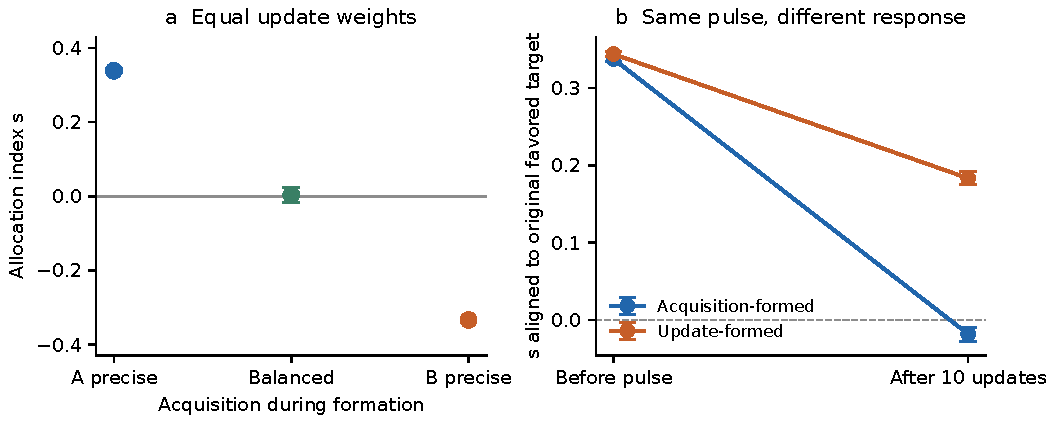
\includegraphics[width=.88\textwidth]{headline_en.pdf}
\caption{A common measured allocation can conceal different adaptation. (a) Acquisition selects specialization with equal loss weights. (b) The matched formation routes receive the same combined opposing pulse. Both move toward the other target, but the acquisition-formed route moves further. Points and intervals summarize 40 seeds; mirrored labels in (b) are averaged within seed. Lines connect endpoints, rather than showing the intervening trajectory.}
\label{fig:headline}
\end{figure}

% P:response3
With inherited Adam, the acquisition-formed route moves further under every pulse (Table~\ref{tab:pulses}). Under the combined pulse, 67.5\% of its checkpoints cross zero within ten updates, compared with 0\% of the update-formed checkpoints (Figure~\ref{fig:headline}b). The continuous route difference is 0.1951. Resetting Adam reduces it to 0.0103, within the pre-specified $\pm0.02$ margin. The other pulses show the same reduction. Thus inherited optimizer state strongly modifies a response difference that selected endpoint measurements and neutral continuation did not reveal.

\begin{table}[t]
\centering\small
\caption{Route difference in specialization lost after ten opposing updates. Brackets give 95\% seed-bootstrap intervals. All inherited-state intervals lie above $+0.05$, and all reset intervals lie inside $\pm0.02$, meeting their respective pre-specified criteria.}
\label{tab:pulses}
\begin{tabular}{lcc}
\toprule
Pulse & Adam inherited & Adam reset\\
\midrule
Acquisition only & $0.1668\ [0.1601,0.1736]$ & $0.0011\ [-0.0010,0.0035]$\\
Update only & $0.1510\ [0.1456,0.1562]$ & $0.0120\ [0.0093,0.0149]$\\
Combined & $0.1951\ [0.1880,0.2021]$ & $0.0103\ [0.0079,0.0129]$\\
\bottomrule
\end{tabular}
\end{table}

% P:response4
This result applies to the two-target network and the ten-update pulses. A separate linear measure of representation similarity (CKA) averages 0.927, and the model parameters are not identical. Resetting Adam leaves those model differences intact. The small reset contrast identifies response equivalence at this ten-update horizon. The zero-crossing rates likewise describe the brief pulse; Section~\ref{sec:time} examines longer common learning.

\section{How retained state changes adaptation}
\label{sec:mechanism}
\subsection{Exchange identifies a second-moment effect}
% P:mechanism1
Adam retains a signed-gradient average $m$ and a squared-gradient average $v$ \citep{kingma2015adam}. The latter sets a separate adaptive scale for each parameter. To test these components directly, we exchange $m$ or $v$ between route endpoints while holding each recipient's weights and optimizer step count fixed. Corresponding parameter coordinates are available because both routes descend from the same ancestor.

% P:mechanism2
In an independent 40-seed comparison, exchanging $m$ leaves the mean response contrast nearly unchanged, with the change inside the pre-specified margin. Exchanging $v$ changes the route contrast from $+0.1968$ to $-0.1265$ (Figure~\ref{fig:moments}a). Both estimates' intervals exclude zero in opposite directions (Appendix~\ref{app:optimizer}). The recipient's second-moment state therefore changes which route is more susceptible. This intervention identifies a causal modifier acting together with the recipient weights and subsequent gradients; it measures the combined ten-update response.

% P:mechanism5
A within-route control holds acquisition, mini-batches, update count, and mean target loss weight fixed. One schedule uses weight 0.80 throughout 500 updates; the other uses 1.00 and 0.60 for 250 updates each in randomized order. The endpoint criteria again pass. The constant schedule then moves further under the common pulse by 0.0324 ($[0.0294,0.0354]$). Exchanging $v$ reverses the contrast to $-0.0141$, while resetting Adam reduces it to 0.0046, inside $\pm0.01$ (Figure~\ref{fig:moments}b). Different acquisition-versus-update labels are therefore unnecessary for this response pattern: equal average loss weights can conceal different optimizer states and later responses. Variability and realized sequence change jointly in this control.

\begin{figure}[t]
\centering
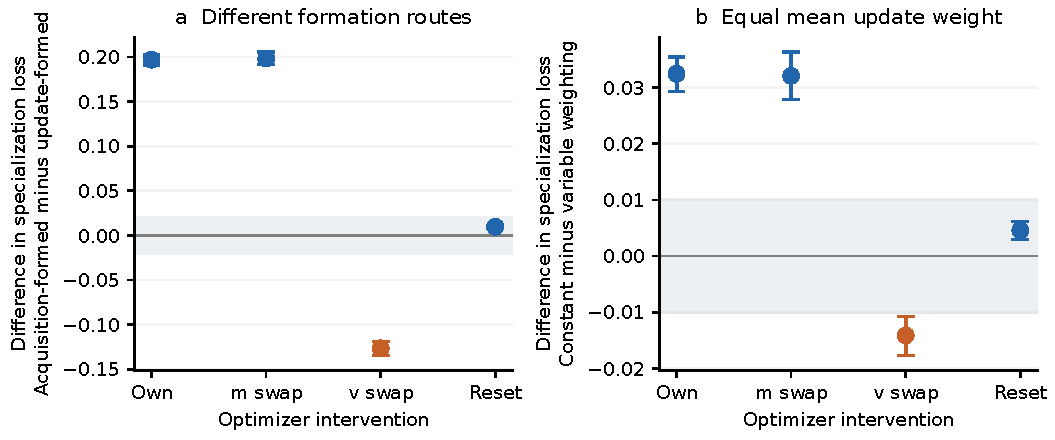
\includegraphics[width=.88\textwidth]{moments_en.pdf}
\caption{Second-moment exchange reverses two short-horizon response contrasts. (a) Acquisition-formed minus update-formed specialization loss. (b) Constant-minus-variable weight-history contrast at fixed acquisition and mean loss weight. Shaded bands show the respective pre-specified equivalence margins ($\pm0.02$, $\pm0.01$). Intervals are paired seed-bootstrap intervals; each comparison uses 40 disjoint confirmatory seeds.}
\label{fig:moments}
\end{figure}

\subsection{Scale, location, and movement}
% P:mechanism3
The exchange raises a more specific question: does one route simply receive a larger average adaptive scale? In a prospective follow-up on 40 new seeds, the inherited-state contrast is 0.1907, reproducing the earlier 0.1951 and 0.1968 estimates. We define $\bar a_v$ as the mean of Adam's bias-corrected inverse-second-moment scaling terms across parameters. This quantity describes the scaling supplied by $v$; an actual update also uses the first moment and current gradient.

% P:mechanism4
Equalizing $\bar a_v$ while preserving each route's coordinate pattern reduces the response difference from 0.1907 to 0.0875. Replacing the pattern by a scalar value gives 0.1251; combining scalarization with a common scale gives 0.0395 (Figure~\ref{fig:timecourse}a). Exchanging the other route's pattern while holding $\bar a_v$ common changes the difference to $-0.0110$. Average scaling thus accounts for part of the response contrast, while coordinate pattern also changes the recipient's response at that common mean. This comparison equalizes a mean inverse-scaling quantity, not the actual update norms throughout the pulse.

% P:mechanism8
A movement-controlled intervention tests whether unequal global path lengths suffice to explain the contrast. At each update, the four branches (two routes, with own or exchanged $v$) receive the geometric mean of their proposed update norms while preserving their directions. With own $v$, the contrast falls from 0.1907 to 0.0303, approximately 84\% under this rule; with exchanged $v$ it is 0.0072, leaving a paired exchange effect of 0.0231. This is a reduction under a different learning rule, rather than the fraction of natural-Adam response causally mediated by movement. The remaining exchange effect shows that equal global movement still permits different reallocation (Table~\ref{tab:ivfmechanism}).

% P:mechanism9
The location of adaptive scaling matters more than its share of total $v$. In acquisition-formed checkpoints, the first encoder layer contains only 5.9\% of total $v$, yet exchanging that layer reduces the contrast from 0.1907 to 0.0115. The heads contain 66.2\%, yet exchanging their $v$ leaves 0.1911. Second-layer exchange leaves 0.0611 (Table~\ref{tab:ivfmechanism}). These interventions retain recipient weights and all other optimizer components. They locate effective interventions in the encoder; their non-additive effects prevent assigning independent causal shares to layers.

\subsection{Formation connects gradient conflict to retained state}
\label{sec:forming}
% P:formationstory
Why is the acquisition route's encoder second moment small? Logging the original 500-update histories reproduces all 160 saved endpoints exactly. The task gradients often point in opposing directions: their negative interaction cancels 94\% and 93\% of the accumulated weighted individual-square sums in the two encoder layers, versus 28\% and 25\% in the update route. The individual-square sums themselves are larger under acquisition. The small second moment therefore reflects cancellation as well as a substantial remaining contribution from the balanced ancestor. This accounting follows actual evolving weights and inputs (Appendix~\ref{app:formationlogs}).

% P:projectionmain
We next alter formation using a two-task PCGrad projection on shared-encoder gradients \citep{yu2020gradient}. When the two weighted gradients conflict, each is projected off the opposing direction; head updates remain unchanged in form. A locally fixed protocol uses 40 new seeds and retains the original acquisition and update routes as controls. Projection raises the acquisition encoder's final second-moment sum by a factor of $1.423\;[1.386,1.459]$ and lowers its mean inverse scale to $0.713\;[0.705,0.721]$ of the original. Transplanting only this projected-history $v$ into the original acquisition recipient changes its ten-update response by $-0.0472\;[-0.0489,-0.0455]$ (Figure~\ref{fig:projection}).

% P:projectionmagnitude
Projection shrinks individual gradients while increasing the squared norm of their sum through reduced cancellation, yet final $v$ remains below the update route (Figure~\ref{fig:projection}a). Because magnitude and interaction change together, it does not partition the original state difference into cancellation and observation-quality contributions.

% P:projectioninterpret
The crossed transplant fixes each recipient while changing $v$: both respond less to projected-history $v$ at ten updates. Projection also changes weights and $m$, and fails endpoint matching. Its total effect therefore supplies neither a matched-endpoint replication nor a natural mediation fraction. It establishes that changing formation produces a different $v$ that alone changes a fixed recipient's response. At 50 updates the donor effects are small and positive. Appendix~\ref{app:projection} gives the factorial comparison, failed criteria and secondary horizon.

\begin{figure}[t]\centering
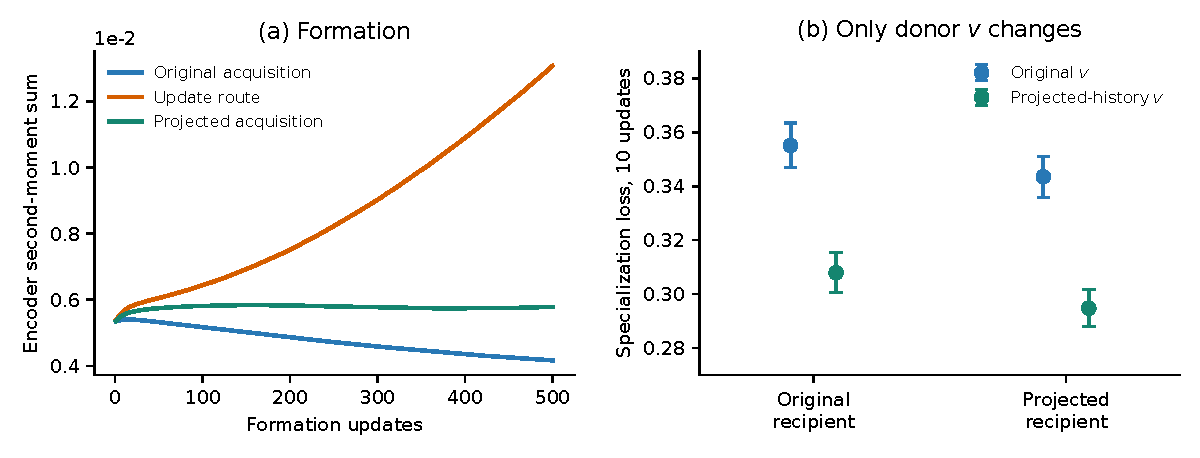
\includegraphics[width=.94\textwidth]{../figures/projection_en.pdf}
\caption{Formation intervention and a fixed-recipient test. (a) Mean encoder second-moment sum during formation in 40 new seeds. (b) Ten-update specialization loss for the two acquisition recipients with original or projected-history second moments. Within each recipient, weights, first moment, and step count are fixed before the pulse; only $v$ changes. Error bars are paired seed-bootstrap 95\% intervals.}
\label{fig:projection}
\end{figure}

\section{The effect has a time scale and a limited scope}
\label{sec:time}
% P:time1
A small difference immediately after reset could still grow during continued learning. We therefore extend the opposing intervention to 500 updates under inherited Adam, fresh Adam, or momentum-free SGD. SGD's common learning rate is calibrated within each seed and target direction using first-batch inherited-Adam update norms and gradient norms, then held fixed; allocation responses are not used for calibration. All three continuations start from the Adam-formed route endpoints.

% P:time2
Inherited Adam produces its largest route differences after 10--20 updates. Fresh Adam gives 0.0096 at update 10 but 0.0274 at update 50; calibrated SGD gives 0.0123 at update 10, 0.0433 at update 50, and 0.0309 at update 100 (Figure~\ref{fig:timecourse}b). The update-50 intervals for fresh Adam and SGD lie above 0.02. That margin was fixed for the ten-update test and is only a reference for later points. The observations show delayed route differences after inherited Adam state has been removed, implicating differences retained on the model side without identifying their specific parameter or geometric source.

% P:time3
The route contrasts shrink toward zero by update 500. Under inherited Adam, the endpoint allocation difference is $-0.00045$ ($[-0.00146,0.00057]$). This endpoint difference is distinct from the difference in change since formation, because the starting measurements were close rather than identical. The inherited-minus-fresh response contrast also changes sign by update 50, so the inherited trajectory is not described by adding a fixed nonnegative fast component to the fresh-Adam trajectory. Within this common opposing condition, optimizer state changes the timing and magnitude of reallocation; the large early difference does not imply a persistent allocation gap.

\begin{figure}[t]
\centering
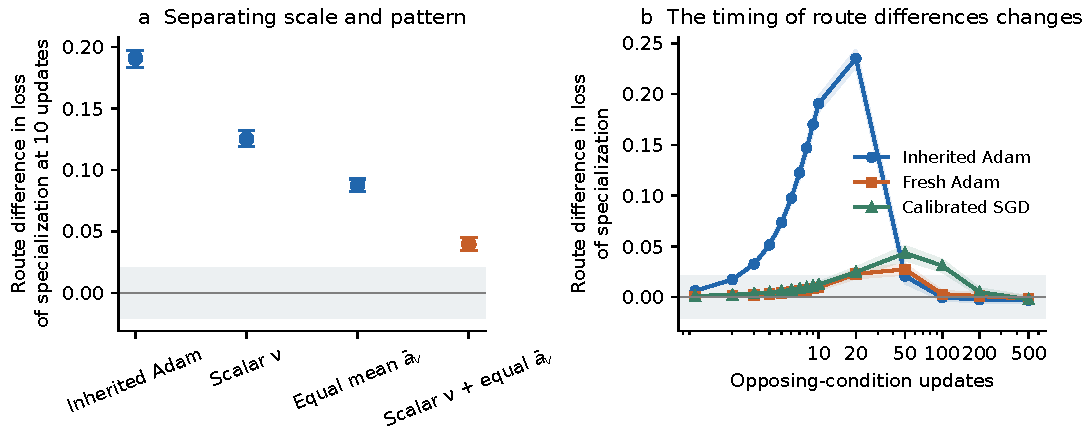
\includegraphics[width=.88\textwidth]{timecourse_en.pdf}
\caption{Scale/pattern interventions and observation horizon resolve different parts of the response. (a) Ten-update route contrast after retaining inherited state, scalarizing $v$, equalizing $\bar a_v$, or both. (b) Continued common opposition under inherited Adam, fresh Adam, or calibrated SGD. The band at $\pm0.02$ refers to the ten-update equivalence margin; later points have no pre-specified decision rule at that margin. Means and 95\% paired seed-bootstrap intervals use 40 new seeds.}
\label{fig:timecourse}
\end{figure}

% P:generalization
Extension IV-F tests the comparison on 32 new paired seeds under changes in hidden width, activation, target correlation, second-moment decay, and formation duration. All nine distinct settings meet the five endpoint tolerances and show a positive common-scale pattern effect (Table~\ref{tab:claims}). This effect subtracts the swapped-pattern route contrast from the own-pattern contrast at the common $\bar a_v$. Reversal and reset equivalence hold in fewer settings. For example, width 64 retains reversal but leaves a reset interval wholly above 0.02. The component effect therefore transfers more broadly than either stronger response pattern.

% P:durationnew
Longer formation does not produce one universal scaling trend. At every tested $\beta_2$, own-state contrasts are larger after 1,500 than 500 updates, and every 1,500-update reset interval exceeds 0.02. At $\beta_2=0.9$, reset increases the contrast at both durations: inherited state can attenuate a route difference. Saved checkpoints show that the acquisition/update mean-inverse-scale ratio grows with duration at 0.999 but falls at 0.9 and 0.99. The 500-update cancellation mechanism thus does not explain the full grid through a uniformly widening scale ratio (Appendix~\ref{app:extension}).

% P:vbmain
Does the component effect depend on having only one alternative target? We form acquisition- and update-driven histories for three symmetric Gaussian targets and test all six ordered changes of favored target. Eight pilot seeds calibrate endpoint measurements without observing adaptation; 40 new seeds test bottleneck dimensions two and three. The response is the decrease in the pairwise allocation index for the original and destination targets, retaining all three reconstruction errors. Both capacities meet all eight mean endpoint criteria. Exchanging $v$ reverses the ten-update route contrast, and exchanging its pattern at a common $\bar a_v$ changes the contrast at both capacities (Tables~\ref{tab:claims} and~\ref{tab:vb}). Reset equivalence holds at dimension two; at dimension three its interval crosses the $+0.02$ boundary and remains unresolved (Appendix~\ref{app:threeadapt}).

% P:naturalnew
The room-sensor extension tests unequal real measurement distributions while retaining the controlled reconstruction task: each room supplies temperature and humidity, so three two-variable targets can replace the Gaussian targets without redesigning the intervention \citep{candanedo2017data,candanedo2017dataset}. Both capacities retain a common-scale pattern effect, but independent confirmation fails endpoint matching (Table~\ref{tab:claims}). This is evidence that the component effect survives this change of input distribution; it is not a matched-endpoint demonstration on natural data. One house and fixed chronological blocks also leave between-building and task generalization untested (Appendix~\ref{app:natural}).

\begin{table}[t]
\centering\small
\caption{Ten-update claims across 13 distinct extension settings. Y: criterion satisfied; N: an interval establishes failure; ?: unresolved. Endpoint matching requires every measurement interval inside its tolerance. Common-scale pattern effect requires a positive interval; reversal requires own positive and exchanged-$v$ negative intervals; reset equivalence requires its interval inside $\pm0.02$. Individual 95\% intervals are used; this inventory is not a success-rate estimate over a population of settings. IV-F has 32 shared seeds; V-B and V-C each have 40, shared across capacities. Baseline occurs only once. Reversal here is a sign criterion; the separate pre-specified requirement that the own-contrast interval exceed $+0.05$ is not met by the two-dimensional room-sensor setting.}
\label{tab:claims}
% P:claimstable
\begin{tabular}{lcccc}
\toprule
Setting & Endpoints & \shortstack{Common-scale\\pattern effect} & Reversal & \shortstack{Reset\\equivalence}\\
\midrule
Baseline ($\beta_2=0.999$, 500) & Y & Y & Y & Y\\
Width 64 & Y & Y & Y & N\\
ReLU & Y & Y & Y & Y\\
$\rho=0$ & Y & Y & Y & Y\\
$\beta_2=0.9$, 500 & Y & Y & N & N\\
$\beta_2=0.99$, 500 & Y & Y & Y & Y\\
$\beta_2=0.9$, 1500 & Y & Y & N & N\\
$\beta_2=0.99$, 1500 & Y & Y & N & N\\
$\beta_2=0.999$, 1500 & Y & Y & Y & N\\
Gaussian, $d_Z=2$ & Y & Y & Y & Y\\
Gaussian, $d_Z=3$ & Y & Y & Y & ?\\
Room sensors, $d_Z=2$ & N & Y & Y & Y\\
Room sensors, $d_Z=3$ & N & Y & ? & Y\\
\bottomrule
\end{tabular}
\end{table}

\section{Implications}
\label{sec:scope}
% P:scope1
The result gives a concrete way to audit continued learning. Measure current specialization, apply the same future learning condition, and test which persistent components alter the response. In this construction, equivalent mean reconstruction measurements coexist with a large early contrast that can be reversed by exchanging $v$. Mean adaptive scale explains only part of that contrast. The equal-mean loss-weight control further shows that average task emphasis can conceal different retained states and responses. Together, these comparisons connect optimizer memory to the reallocation of information within a shared representation.

% P:scope2
A concrete application is evaluating a checkpoint before resuming training on a changed task. The comparison suggests testing a common continuation with optimizer state inherited and reset, alongside current readout quality. In the present system these choices change the timing and magnitude of adaptation. Whether the same diagnostic improves decisions in fine-tuning requires validation on the target task, including its eventual performance.

% P:scopecompact
The matched evidence concerns small bottleneck networks, two or three Gaussian targets, prescribed observation/loss histories, and finite continuation horizons. Matching selected mean readouts does not match all model functions or geometry. The component interventions remain interpretable because they hold each recipient fixed at the branch point; transplantation requires corresponding coordinates from a common ancestor. Testing practical checkpoint choices requires target-task evidence, including final performance, rather than treating faster reallocation as inherently better.

\section{Conclusion}
% P:conclusion
Similar measured specialization can conceal latent susceptibility to further learning in the studied two- and three-target Gaussian systems. Component exchange identifies inherited Adam second moments as a causal modifier of early reallocation, with effects beyond mean adaptive scale and, in the two-target control, beyond global update norm. Formation records and projection-plus-transplant interventions connect the gradient history to a second moment that changes the recipient response. The natural sensor extension retains component effects but fails endpoint matching, separating transfer of the intervention effect from transfer of the concealed-response claim. Reset equivalence and sign reversal depend on capacity, learning conditions, and horizon. Current readout quality, persistent training state, and subsequent learning conditions jointly determine what an adaptation comparison reveals.

\section*{Reproducibility statement}
% P:repro
\ifpublicrelease
Code and generated data are available at \url{https://github.com/culturegeek/matched-specialization-different-adaptation} (\href{https://github.com/culturegeek/matched-specialization-different-adaptation/releases/tag/v1.5.2}{v1.5.2}).
\else
An anonymized code and data archive accompanies this manuscript as supplementary material.
\fi
The archive contains source code, locally frozen plans, seed-level trajectories, checkpoints, and audit scripts for the studies reported here and the wider research program. Code uses MIT; generated data and documentation use CC BY 4.0. The redistributed UCI sensor dataset retains its original CC BY 4.0 attribution. Appendix~\ref{app:status} maps claims to files and gives CPU-based integrity, numerical, figure-generation, and training-reproduction checks.

\section*{Broader impact statement}
% P:impact
The work supplies controlled comparisons for examining shared representations whose input access and learning histories vary over time. Applications to deployed systems require direct validation of the interventions and measurements in those settings.

\section*{AI assistance statement}
% P:ai
Generative AI systems were used extensively to propose most experiment designs and follow-up analyses, implement and execute experiments, analyze outputs, survey literature, and draft and translate the manuscript. The human author initiated the broader research program, commissioned this empirical study, authorized its continuation at major decision points, reviewed the evidence and claims, and accepts responsibility for the paper and its public release.

\bibliography{references}
\bibliographystyle{tmlr}
\FloatBarrier
\appendix
\section{Measurement and paired inference}
\label{app:measurement}
% P:measurementcompact
The central network is $6\to32\to2$ with tanh after both encoder layers and two linear heads. Training/probe/test sample counts are $3072/768/1536$, batch size 256, Adam learning rate 0.002, $(\beta_1,\beta_2)=(0.9,0.999)$, $\epsilon=10^{-8}$, weight decay $10^{-5}$, and readout ridge coefficient $10^{-3}$. Each seed supplies a common ancestor and paired data/batches. Fresh linear readouts fit on unused probe data and evaluate on separate test data. Common high- and low-precision inputs distinguish learned readout quality from momentary observation quality.

% P:appmargins
The formation tolerances are $\pm0.02$ for aligned $s$, target and non-target errors, and their sum, and $\pm0.01$ for low-precision aligned $s$. IV-D uses response bands of $\pm0.02$ for neutral continuation and reset responses, and $\pm0.05$ for inherited-state pulses. IV-E uses $\pm0.02$ for the change under $m$ exchange and for the reset response; the within-route update-history control uses $\pm0.01$ for its reset response. These criteria apply to intervals for mean paired differences.

% P:appmarginrule
IV-D classifies a contrast as equivalent when its 95\% interval lies wholly inside the specified band, practically different when it lies wholly beyond either boundary, and unresolved otherwise. All three inherited-state pulse intervals lie wholly above $+0.05$ (Table~\ref{tab:pulses}), indicating positive, practically meaningful route differences. All reset-pulse intervals lie inside $\pm0.02$.

% P:appmarginorigin
IV-D calibrates route strength on pilot seeds 8000--8015 and fixes the tolerances before seeds 8100--8139. IV-E uses pilot seeds 9000--9015 to set response criteria before seeds 9100--9139; the within-route control explicitly uses pilot seeds 9200--9215 to set its response criteria and equivalence margin before seeds 9300--9339. The plans document these operational choices but do not derive the margins from an independent practical-error criterion. Equivalence therefore denotes agreement at the stated resolutions in these synthetic comparisons.

% P:endpointpredictioncompact
Endpoint equivalence is about intervals for selected mean paired measurements, not equality of every seed pair or of all model functions. Representation similarity (CKA) averages 0.927. A saved-data check predicts ten-update response contrasts from target error, other-target error, and low-precision allocation differences. Leave-one-seed-out error ratios relative to a training-mean predictor are 1.118, 1.023, and 0.984 in three independent 40-seed cohorts. The measured residual features therefore give little linear predictive improvement; this does not remove confounding by unmeasured geometry. The full held-out predictions are archived.

\section{State interventions and continuation}
\label{app:optimizer}
% P:appopt1
IV-D uses 40 confirmatory seeds and two mirrored directions per seed. Mean aligned $s$ is 0.3375 after acquisition-driven formation and 0.3439 after update-driven formation; corresponding target/non-target errors are 0.4034/0.8144 and 0.4000/0.8198. The route strengths are pilot-calibrated, not fitted to the confirmatory endpoints. Neutral-continuation integral differences are $-0.0025$ ($[-0.0064,0.0013]$) with Adam inherited and $-0.0018$ ($[-0.0068,0.0030]$) after reset. Carried-minus-reset response interactions for acquisition, update, and combined pulses are 0.1657, 0.1390, and 0.1848, each exceeding the pre-specified 0.08 criterion.

% P:appopt2
In IV-E, the own-minus-$m$-exchange change is $-0.0014$ ($[-0.0044,0.0018]$), inside $\pm0.02$. The acquisition-formed route's total second moment is 0.5577 times the update-formed route's, while the mean coordinate-wise inverse-second-moment scaling factor is 1.950 times larger. This scaling factor is not the actual parameter-update ratio: Adam's update also depends on the first moment, current gradient, and bias correction. Table~\ref{tab:components} gives the main component contrasts.

\begin{table}[h]
\centering\small
\caption{Combined-pulse response contrasts under component interventions. IV-E compares acquisition-formed minus update-formed routes; the control compares constant minus variable update-weight histories. Each uses 40 disjoint confirmatory seeds.}
\label{tab:components}
\begin{tabular}{lcc}
\toprule
Component condition & IV-E route contrast & Equal-mean update-history control\\
\midrule
Own state & $0.1968\ [0.1910,0.2029]$ & $0.0324\ [0.0294,0.0354]$\\
Exchange $m$ & $0.1982\ [0.1912,0.2054]$ & $0.0321\ [0.0277,0.0362]$\\
Exchange $v$ & $-0.1265\ [-0.1348,-0.1183]$ & $-0.0141\ [-0.0176,-0.0110]$\\
Reset & $0.0097\ [0.0078,0.0117]$ & $0.0046\ [0.0031,0.0062]$\\
\bottomrule
\end{tabular}
\end{table}

% P:withinroutecompact
The equal-mean history control uses constant favored-target weight 0.80 or a random ordering of 250 updates each at 1.00 and 0.60, with acquisition, batches, and total updates fixed. Pilot and confirmation use disjoint seeds. Every endpoint criterion passes; Table~\ref{tab:components} reports the response contrasts. Variability and sequence change jointly. This control shows that different acquisition/update route labels are unnecessary for the effect, while leaving an isolated order effect unidentified.

% P:scaleprocedure
For step count $t$ and $P$ parameters, the mean adaptive scale is
\begin{equation}\bar a_v=P^{-1}\sum_j\frac{\eta}{\sqrt{v_j/(1-\beta_2^t)}+\epsilon}.\end{equation}
The common target is the geometric mean of the two routes' original values. Pattern-preserving normalization replaces $v$ by $cv$, solving for positive $c$ by 80 bisection iterations including $\epsilon$. Pattern exchange transplants $v$ first, then normalizes it. Scalarization instead sets all $v_j=(\eta/a_\ast-\epsilon)^2(1-\beta_2^t)$, using either the common or own scale. Recipient weights, $m$, and step count remain fixed. Relative scale errors are below $2\times10^{-6}$. A common ancestry supplies corresponding coordinates.

% P:continuationcompact
The follow-up uses seeds 20000--20039. For momentum-free SGD, one common learning rate per seed/direction is the geometric mean of the two first-batch Adam-update norms divided by the corresponding regularized-gradient norms; response measurements are not used. It is then held fixed (0.0194--0.0529). The primary ten-update bands do not define confirmatory gates at later horizons. At 50 updates fresh-Adam and SGD contrasts have intervals $[0.0227,0.0321]$ and $[0.0368,0.0499]$. By 500 updates, measured allocation endpoints approach each other; convergence of complete model states is untested. The separate ten-update-pulse-then-neutral continuation likewise reduces the endpoint gap, from 0.06197 at update 50 to 0.00984 at 510.

\section{Locating, recording, and perturbing the retained state}
\label{app:mechanism}
\subsection{Layer and movement controls}
\label{app:layers}
% P:movementprocedure
Layer exchange changes only the named layer's $v$, including its biases. The movement control runs four branches (two routes, own/exchanged $v$) jointly. At each step their proposed Euclidean update norms determine a shared geometric-mean norm. Each update is rescaled without changing its direction; moments continue evolving at the actual positions. Achieved relative discrepancies are below $2\times10^{-6}$. These interventions change the learning rule and do not identify natural-Adam mediation fractions or additive layer contributions.

\begin{table}[t]
\centering\small
\caption{Layer and movement interventions on 40 saved seed pairs. Layer rows exchange only the named layer's $v$; equal-movement rows apply the joint norm-control rule.}
\label{tab:ivfmechanism}
% P:appfmechanismtable
\begin{tabular}{lr}
\toprule
Intervention & Route contrast [95\% CI]\\
\midrule
Own & $0.1907\;[0.1837,0.1976]$ \\
First encoder layer & $0.0115\;[0.0060,0.0171]$ \\
Second encoder layer & $0.0611\;[0.0558,0.0665]$ \\
Both heads & $0.1911\;[0.1838,0.1978]$ \\
All parameters & $-0.1183\;[-0.1264,-0.1099]$ \\
Equal movement, own & $0.0303\;[0.0269,0.0338]$ \\
Equal movement, exchanged & $0.0072\;[0.0040,0.0104]$ \\
\bottomrule
\end{tabular}

\end{table}

\subsection{Accounting for the formation history}
\label{app:formationlogs}
\label{app:headgrad}
% P:loggingdesigncompact
The exploratory replay retains the original 40 follow-up seeds, two directions and two routes, with all inputs, batches, loss weights and Adam settings unchanged. Separate head gradients are recorded before the original weighted backward pass. All 160 endpoints reproduce bitwise in the recorded environment. If $g_f,g_o$ are the unweighted head gradients, then the squared weighted gradient separates into individual squares, a cross term and weight-decay terms. Accumulating each with the same $\beta_2$ gives, coordinate by coordinate,
\begin{equation}v_T=\beta_2^T v_0+S_T+C_T+R_T+E_T.\end{equation}
Here $S_T$ accumulates $w_f^2g_f^2+w_o^2g_o^2$, $C_T$ accumulates $2w_fw_og_fg_o$, $R_T$ contains coupled weight decay, and $E_T$ is the floating-point remainder. Cancellation is $-C_T/S_T$ after summing coordinates within a layer; directions are averaged within seed. This is an arithmetic decomposition of the observed trajectory.

% P:formationlogresult
Mean cancellation is stronger in the acquisition route throughout formation (Figure~\ref{fig:formationlogs}). At update 500, $-C/S$ is $0.942\;[0.939,0.945]$ and $0.930\;[0.927,0.934]$ in its first and second encoder layers, compared with $0.284\;[0.271,0.298]$ and $0.252\;[0.238,0.268]$ in the update route. The corresponding final acquisition/update $v$ ratios are $0.242\;[0.230,0.255]$ and $0.340\;[0.321,0.361]$. The retained ancestor contributes about 64\% and 79\% of acquisition-route final $v$, versus 16\% and 28\% for the update route, averaging direction-specific fractions within seed. The mean accumulated individual-square sum $S$ is larger under acquisition in both layers. Thus the small final state combines strong cancellation of newly accumulated task gradients with a substantial inherited contribution.

% P:paireds
Paired seed differences quantify the difference in individual-square sums. Acquisition-minus-update $S_T$ is $0.000931\;[0.000831,0.001035]$ in layer one and $0.000355\;[0.000088,0.000636]$ in layer two. Both paired intervals are positive, with a smaller difference in the second layer.

% P:strata
Observation strata help locate the accumulation. In the first layer, acquisition updates (favored target always precise) have mean cosine about $-0.94$ and cancellation 0.94. Update-route steps with the favored target precise have $-0.81$ and 0.48, whereas other-target-precise steps have about $-0.08$ and 0.06. In updates 251--500 the latter cross term becomes positive (cosine about $+0.11$, cancellation $-0.12$), consistent with the decline in accumulated cancellation after its early peak. These are conditional observations along different evolving states and loss weights, not an isolated causal effect of observation precision.

\begin{figure}[ht]
\centering
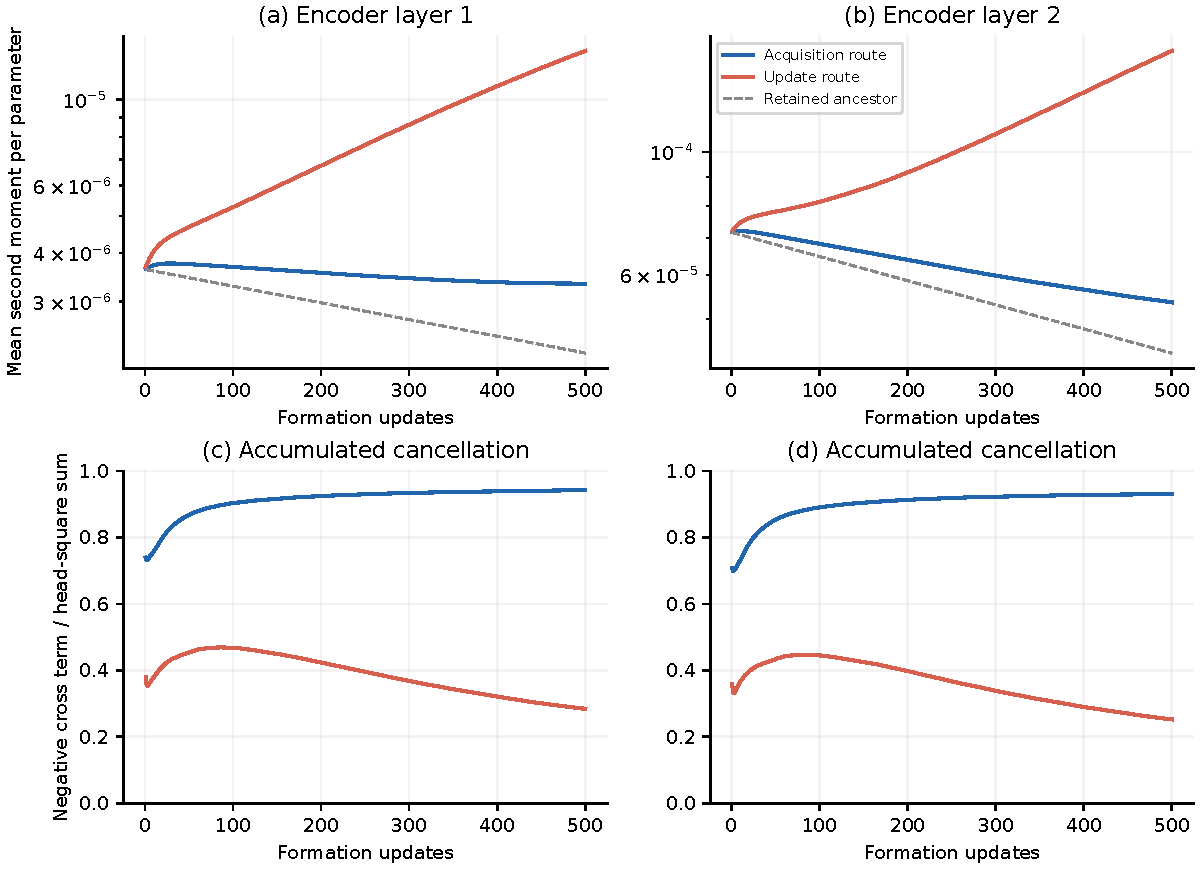
\includegraphics[width=.86\textwidth]{formation_logging_en.pdf}
\caption{Formation-time accounting on the original 40 paired seeds. Top: mean second moment per parameter in each encoder layer; dashed curves show the discounted shared ancestor. Bottom: mean accumulated cancellation fraction $-C/S$ along each route's actual observations and loss weights. Curves average both directions within seed and then seeds; interval estimates for the final values appear in the text.}
\label{fig:formationlogs}
\end{figure}

% P:endpointdiagnostics
Common-input endpoint probes provide a complementary diagnostic. Under both-high precision the acquisition route has larger individual head gradients but a smaller equally weighted sum; the favored-precise probe instead has first-layer cosines $-0.940/-0.835$. The effect changes with input precision and loss weights. Across seeds, cosine-response associations are unresolved, while the log norm ratio has a positive exploratory association; these estimates do not separate gradient and optimizer causes. All probe conditions, norms, correlations and independent chain-rule checks remain in the reproduction archive.

\subsection{Projection followed by crossed state transplantation}
\label{app:projection}
% P:pcmethod
A new locally specified test uses seeds 38000--38039, with seed 37999 reserved for implementation checks. Each seed and favored direction share the ancestor, training examples, batch order and 500-update schedule. We retain native acquisition and update formation, and add projected acquisition. For the two weighted shared-encoder gradients $u,v$, if $u^\top v<0$, set
\begin{equation}u'=u-\frac{u^\top v}{v^\top v}v,\qquad v'=v-\frac{u^\top v}{u^\top u}u.\end{equation}
Both expressions use the original vectors. The encoder receives $u'+v'$; each head retains its weighted task gradient, and Adam adds weight decay normally. This shared-encoder implementation of PCGrad changes both direction and magnitude. It removes conflicting components without holding all other properties of formation fixed.

% P:pcinference
At formation end, native and projected acquisition recipients each receive native or projected $v$, giving a $2\times2$ transplant. Within recipient, model weights, $m$, step count and all pulse inputs are fixed. The unchanged update route provides a reference. The same opposing pulse runs for 50 updates; ten is primary and 50 secondary. Both directions are averaged within seed; all 40 seeds enter 10,000 paired bootstrap resamples (random stream 2026101704). Log ratios are averaged over directions within seed and then across seeds. The pre-run source hashes, all trajectories and all criteria are retained.

\begin{table}[ht]\centering\small
\caption{Crossed second-moment transplants: specialization loss after ten updates. Each row fixes recipient weights and first moment. Intervals use 40 paired seeds.}
\label{tab:projection}
% P:projectiontable
\begin{tabular}{lcc}\toprule
Recipient & Native $v$ & Projected-history $v$\\
\midrule
Native acquisition & $0.3551\;[0.3469,0.3634]$ & $0.3079\;[0.3007,0.3154]$\\
Projected acquisition & $0.3435\;[0.3358,0.3512]$ & $0.2948\;[0.2880,0.3016]$\\
\bottomrule\end{tabular}\end{table}

% P:pcfailure
The original acquisition/update comparison satisfies every endpoint band in this cohort. Projection changes the recipient: under the locally specified $\pm0.02$ bands, only target error and low-precision allocation satisfy equivalence; aligned allocation, other-target error and total error do not. The projected-minus-update aligned-allocation difference is $0.0416\;[0.0388,0.0442]$. Projected-own minus native-own response is $-0.0603\;[-0.0638,-0.0570]$; the projected-$v$ donor effect on the projected recipient is $-0.0487\;[-0.0503,-0.0470]$. The two donor effects have the same direction, but their ratio to the total formation effect is not a causal mediation proportion.

% P:projection50
At 50 updates, projected-history $v$ changes the native and projected recipients' responses by $+0.0029\;[0.0025,0.0032]$ and $+0.0021\;[0.0017,0.0026]$, respectively. The total projected-own minus native-own contrast is $+0.0440\;[0.0417,0.0461]$. The secondary horizon therefore reverses both the small donor effects and the total formation contrast; a reduction after ten updates is not a persistent reduction.

% P:projectiondecomposition
Exploratory reaggregation of the saved formation traces uses the same exponential weights as $v$. Post/pre ratios on the projected trajectory are 0.117 for the individual-square sum and 1.844 for the squared norm of their sum: individual gradients shrink while their sum grows. Ratios are geometric means over 40 seeds after log-averaging directions within seed. These describe visited states, not an unobserved unprojected trajectory; complete results remain archived.

\section{Regime and target extensions}
\label{app:extension}
% P:regimedesign
Nine distinct settings reuse seeds 32000--32031: the baseline, width 64, ReLU, independent targets, and the $3\times2$ decay/duration grid sharing one baseline. Other settings retain the original protocol, including five endpoint tolerances and six pulse modes. All settings satisfy endpoint tolerances and positive common-scale pattern effects. Width 64 fails reset equivalence. Table~\ref{tab:claims} separates sign reversal from the positive $+0.05$ response-size criterion; Table~\ref{tab:ivfbeta} supplies the decay/duration estimates. This finite selected grid characterizes tested conditions, not the prevalence of an effect over all networks.

\begin{table}[ht]
\centering\small
\caption{Decay and duration grid, 32 paired seeds per setting. Common-scale pattern effect is the route-contrast difference before minus after $v$ exchange at common $\bar a_v$. All settings satisfy endpoint tolerances.}
\label{tab:ivfbeta}
% P:appfbetatable
\begin{tabular}{llcccc}
\toprule
$\beta_2$ & Formation & Own state & Exchange $v$ & Reset & \shortstack{Common-scale\\pattern effect}\\
\midrule
$0.9$ & 500 & \shortstack{$0.0298$\\$[0.0278,0.0318]$} & \shortstack{$0.0104$\\$[0.0082,0.0127]$} & \shortstack{$0.0373$\\$[0.0342,0.0406]$} & \shortstack{$0.0058$\\$[0.0053,0.0064]$} \\
$0.9$ & 1500 & \shortstack{$0.0764$\\$[0.0736,0.0794]$} & \shortstack{$0.0494$\\$[0.0462,0.0526]$} & \shortstack{$0.1073$\\$[0.1023,0.1123]$} & \shortstack{$0.0120$\\$[0.0111,0.0131]$} \\
$0.99$ & 500 & \shortstack{$0.1385$\\$[0.1329,0.1444]$} & \shortstack{$-0.0720$\\$[-0.0770,-0.0672]$} & \shortstack{$0.0174$\\$[0.0150,0.0197]$} & \shortstack{$0.0673$\\$[0.0625,0.0721]$} \\
$0.99$ & 1500 & \shortstack{$0.2859$\\$[0.2789,0.2925]$} & \shortstack{$0.0297$\\$[0.0204,0.0390]$} & \shortstack{$0.0963$\\$[0.0913,0.1014]$} & \shortstack{$0.1334$\\$[0.1204,0.1448]$} \\
$0.999$ & 500 & \shortstack{$0.1962$\\$[0.1881,0.2043]$} & \shortstack{$-0.1290$\\$[-0.1379,-0.1198]$} & \shortstack{$0.0073$\\$[0.0054,0.0092]$} & \shortstack{$0.1028$\\$[0.0947,0.1109]$} \\
$0.999$ & 1500 & \shortstack{$0.4341$\\$[0.4277,0.4408]$} & \shortstack{$-0.1279$\\$[-0.1416,-0.1139]$} & \shortstack{$0.0574$\\$[0.0529,0.0618]$} & \shortstack{$0.2528$\\$[0.2414,0.2644]$} \\
\bottomrule
\end{tabular}

\end{table}

% P:appfbeta2
The reset column shows what remains after removing inherited optimizer state. At $\beta_2=0.9$, reset contrasts are 0.0373 and 0.1073 after 500 and 1,500 formation updates, larger than their own-state contrasts of 0.0298 and 0.0764. At 1,500 updates all three reset intervals lie above 0.02. Thus reset does not define an additive subtraction of optimizer and model contributions. The grid changes formation trajectories and subsequent adaptation together, so it identifies regime dependence rather than an isolated memory-duration effect. At $\beta_2=0.9$, a paired exploratory comparison confirms reset-minus-own increases of $0.0075\;[0.0059,0.0090]$ and $0.0308\;[0.0282,0.0334]$ for 500 and 1,500 formation updates. Reset changes both moments and the optimizer step count; this contrast does not isolate $v$ alone.

% P:durationratios
Reading all nine settings' saved checkpoints adds no training. In the six-setting decay/duration grid, for $\beta_2=0.9,0.99,0.999$, the 1,500/500 change in the acquisition/update mean-inverse-scale ratio is $0.792\;[0.759,0.827]$, $0.702\;[0.662,0.747]$, and $1.066\;[1.042,1.091]$, respectively. These are paired geometric ratios from 32 seeds with 10,000 bootstrap resamples. Thus the increasing response contrast at every decay rate does not imply an increasing mean-scale ratio at every rate. Layerwise results and all endpoints are retained in the archive.

\subsection{Three Gaussian targets}
\label{app:threeadapt}
% P:appvbdesign
To test whether optimizer-mediated reallocation survives a third competing target, we use a Gaussian construction (V-B): three three-dimensional targets with pairwise correlation 0.35, a $9\to32\to d_Z$ tanh encoder, and three linear heads. For each $d_Z\in\{2,3\}$ and original target $i$, acquisition formation observes $i$ precisely with equal loss weights. Update formation balances precision across targets while assigning $i$ weight $w$ and the others $(1-w)/2$. Both descend from the same 100-update balanced ancestor and train for 600 further updates with Adam. Learning rate, decay, batch size, and train/probe/test counts are $0.002$, $(0.9,0.999)$, 256, and $3072/768/1536$; weight decay is $10^{-5}$ and $\epsilon=10^{-8}$.

% P:appvbcal
Eight pilot seeds (33000--33007) compare $w=0.55,0.60,\ldots,0.95$ using endpoints alone. For each capacity we minimize the largest absolute mean endpoint difference divided by its tolerance. The selected weight is 0.65 at both capacities. Eight measurements align the original target and its two cyclic alternatives: three errors, their sum, two pairwise indices, and the two indices under a low-precision probe. Tolerances are $\pm0.02$, or $\pm0.01$ for low-precision indices. The three original-target labels are averaged within seed in this symmetric construction. Confirmation on seeds 34000--34039 meets every interval-based endpoint criterion at both capacities. These are operational measurement tolerances, not externally validated performance thresholds.

% P:appvbresponse
Each endpoint receives two destination-target pulses, giving all six ordered directions. A pulse observes destination $j$ precisely and weights its loss 0.8, with 0.1 for each other target. Define $s_{ij}=(D_j-D_i)/(D_j+D_i)$ and response $s_{ij}(0)-s_{ij}(t)$. The route contrast subtracts update-formed response from acquisition-formed response. All three errors and centered log-error scores are retained. The six optimizer modes use own state, exchanged $m$, exchanged $v$, fresh Adam, own $v$ at common $\bar a_v$, or exchanged $v$ at the same common scale. Exchanges preserve recipient weights, the other moment, and step count; scale normalization uses the geometric mean of the two original scales and 80 bisection iterations including $\epsilon$.

% P:vbcompact
Ten updates are primary and 50 secondary. All six ordered target directions are averaged within seed; each capacity uses the same 40 confirmation seeds. Individual intervals use 5,000 paired bootstrap resamples. Both capacities satisfy endpoint matching and reversal; reset equivalence remains unresolved at dimension three. Common-scale pattern effects are positive at both capacities (Table~\ref{tab:targets}). At 50 updates, own-state contrasts are approximately 0.0000/0.0069, reset contrasts 0.0255/0.0596, and common-scale effects $-0.0241/-0.0479$. The early positive component effect therefore changes with observation horizon.

\subsection{Unequal room-sensor measurements}
\label{app:natural}
% P:appvcdata
The room-sensor extension (V-C) tests natural cross-target and temporal structure using the UCI Appliances Energy Prediction data \citep{candanedo2017data,candanedo2017dataset}. The source contains 19,735 ten-minute records from one house, January--May 2016. The targets are kitchen temperature/humidity (T1, RH\_1), living-room measurements (T2, RH\_2), and laundry-room measurements (T3, RH\_3). The task reconstructs these recorded values after controlled observation noise; it is neither future forecasting nor the source dataset's appliance-energy benchmark.

% P:appvcsplit
The first 9,867 rows train the model. Four subsequent chronological blocks fit and evaluate pilot readouts (2,816 and 2,817 rows), then fit and evaluate confirmation readouts (1,829 and 1,830 rows). We omit 144 rows at each boundary. Training ends on March 20, pilot evaluation on April 30, and confirmation evaluation spans May 15--27. Means and standard deviations come only from the training block and are fixed thereafter. $D_i$ averages squared error over the room's two training-standardized variables, without normalization by evaluation-block variance. The model's formation and pulse updates use only the training block; fresh readouts use their designated later blocks. Gaps reduce immediate overlap but do not establish temporal independence.

% P:appvcdesign
The encoder becomes $6\to32\to d_Z$ with two-dimensional heads; training settings, precision noise, six directions, six modes, and horizons otherwise follow V-B. Room labels keep their physical meaning. Eight pilot seeds (35000--35007) select a weight separately for each original room and capacity, among $1/3$, 0.40, 0.45, \ldots, 0.95. Selection minimizes the same largest standardized mean endpoint discrepancy, without using pulse responses or confirmation blocks. Selected weights for kitchen/living/laundry are 0.40/0.95/0.75 at dimension two and 0.95/0.95/0.90 at dimension three. Even the best candidates exceed the largest allowed mean discrepancy by factors of 5.30--12.44. The fixed protocol carries these candidates into confirmation without expanding the search.

% P:appvcmatch
Forty new confirmation seeds (36000--36039) again fail endpoint matching. Because rooms are not exchangeable, matching requires all eight criteria for each original room, rather than averaging away room-specific differences. Only 1 of 24 criteria passes at dimension two, and none passes at dimension three. Direct input readouts verify that precise acquisition reduces the designated room's error: gains are 0.1784, 0.4822, and 0.1824 for kitchen, living room, and laundry room. Thus observation control remains effective, while this grid and formation schedule do not yield matched route endpoints. At dimension two, averaging original rooms within seed gives acquisition-minus-update differences of +0.0616 in $s_{01}$ and +0.0238 in its low-precision counterpart: acquisition-formed checkpoints start with greater measured relative specialization on this comparison. These pooled descriptions do not replace the room-specific matching criteria. Since response subtracts the final index from its initial value, this initial difference can contribute to the unmatched route contrast.

% P:vccompact
The same 40 seeds are reused across capacities. At ten updates, both retain a positive common-scale pattern effect (Table~\ref{tab:targets}). Dimension two has sign reversal but fails the separate own-contrast lower bound of $+0.05$; dimension three has an unresolved swapped sign. At 50 updates, own-state contrasts are 0.0842/0.1156 and reset contrasts 0.0124/0.0392. Every interval conditions on the fixed building and time blocks, measuring training/noise-seed variation rather than between-building uncertainty. Endpoint matching remains unsuccessful.

\begin{table}[ht]\centering\small
\caption{Three-target ten-update contrasts. G: Gaussian; S: room sensors. Sensor endpoints are unmatched. All intervals are individual 95\% paired-seed intervals.}
\label{tab:targets}\label{tab:vb}\label{tab:vc}
\begin{tabular}{lcccc}\toprule
Condition & G, $d_Z=2$ & G, $d_Z=3$ & S, $d_Z=2$ & S, $d_Z=3$\\
\midrule
% P:targetown
Own & \shortstack{$0.1945$\\$[0.1906,0.1987]$} & \shortstack{$0.4054$\\$[0.3951,0.4152]$} & \shortstack{$0.0601$\\$[0.0456,0.0741]$} & \shortstack{$0.1170$\\$[0.1024,0.1320]$}\\
% P:targetswap
Exchanged $v$ & \shortstack{$-0.1005$\\$[-0.1054,-0.0955]$} & \shortstack{$-0.2193$\\$[-0.2266,-0.2118]$} & \shortstack{$-0.0254$\\$[-0.0381,-0.0130]$} & \shortstack{$-0.0090$\\$[-0.0232,0.0049]$}\\
% P:targetreset
Reset & \shortstack{$0.0116$\\$[0.0101,0.0132]$} & \shortstack{$0.0203$\\$[0.0178,0.0226]$} & \shortstack{$-0.0076$\\$[-0.0168,0.0017]$} & \shortstack{$0.0046$\\$[-0.0062,0.0152]$}\\
% P:targetpattern
\shortstack{Common-scale\\pattern effect} & \shortstack{$0.0825$\\$[0.0792,0.0860]$} & \shortstack{$0.1541$\\$[0.1479,0.1597]$} & \shortstack{$0.0103$\\$[0.0064,0.0140]$} & \shortstack{$0.0257$\\$[0.0210,0.0306]$}\\
\bottomrule\end{tabular}\end{table}

\section{Reproduction and evidence status}
\label{app:status}
% P:reproductioncompact
The matched comparisons, component and scale/pattern interventions, regime extensions and projection study retain their locally fixed plans and all failed criteria. Formation logging, endpoint diagnostics and saved-data decompositions are exploratory. Time-stamped source hashes document local specifications, not public-registry preregistration.

% P:evidencemap
\texttt{docs/PAPER\_TO\_DATA.md} maps each claim, figure and table to its code and evidence. Formation records and projection transplants are in \texttt{experiments/iv-formation-logging/} and \texttt{iv-cancellation/}. The interval ledger binds every printed interval to a result key and rounding precision. The wider program's studies and unsuccessful analyses retain their complete records and original status in the full archive.

% P:reproenvironment
Follow-up training used Python 3.11.7; formation/projection runs used Python 3.12.14 and NumPy 2.4.6. Both used PyTorch 2.13.0 on single-threaded CPU. Bitwise equality was observed there, not guaranteed across environments. The reproduction runner and both formation audits default to strict equality. Explicit \texttt{-{}-tolerance 1e-6} records tensor-specific bounds, errors and actual bitwise status for replayed floating states; hashes, schedules, steps and transplants remain exact. The README documents cross-version checks. Original logs and locks remain unchanged.



\end{document}
